\section{Lithium teknologi}
Lithium batterier har siden 1973 været under konstant udvikling. Gennem tiden er der opdaget mange forskellige typer for lithium batterier. Målet er, som ved så mange andre typer batterier, at få den højeste kapacitet på mindst mulig plads. Men da der ved lithium batterier er farlige konsekvenser ved dette, skal det det bedste kompromis findes. "Hovednavnet" \space /det mest brugte navn for de mange forskellige typer er bare "lithium-ion" \space men hvis der dykkes lidt dybere ned i kemien ses der at der findes lithium-ion batterier med mange forskellige karakteristika. 

\subsection{Forskel på kemierne}
Den nok mest brugte er dog lithium cobalt oxid-typen ($LiCoO_2$, også kaldt $LCO$) som bruges i f.eks. mobiltelefoner og moderne bærbare computere. Denne type er den mest fleksible i dens fysiske design, men også den farligste. Derfor er det vigtigt at denne type celle har et overvågningskredsløb, da der ellers kan forekomme katastrofale situationer. Disse celler er oftest formet som "bløde puder" \space \textemdash \space altså uden en hård kasse rundt om. Denne teknologi bruges også oftest i lithium ion polymer-varianten, som bliver brugt meget i RC-industrien pga. den høje afladekapacitet og den kompakte form.

\begin{figure}[h]
	\centering
	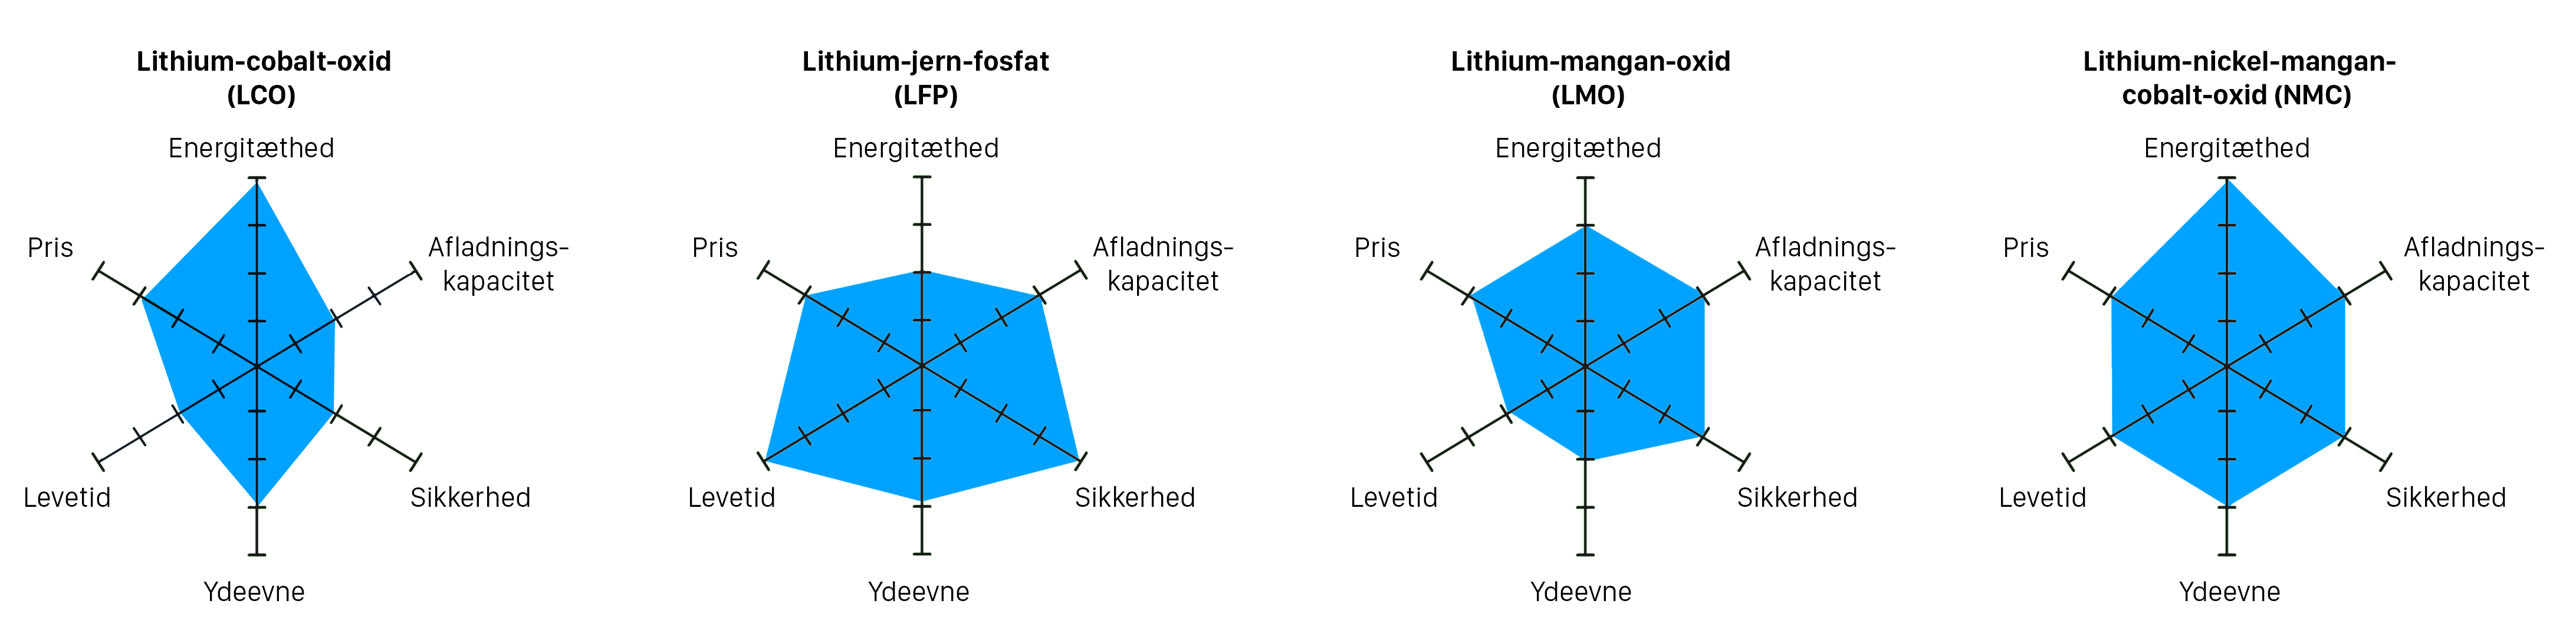
\includegraphics[width=15cm]{billeder/chemical-comparison.png}
	\caption{Sammenligning af de forskellige former for lithium ion celler\protect\footnotemark}
	\label{fig:lithium_variants_comparison}
\end{figure}
\footnotetext{BCG Research forskning i de bedste batterier til el-biler. \url{https://www.bcg.com/documents/file36615.pdf}}

Som der ses på figur \ref{fig:lithium_variants_comparison} sammenlignes de forskellige typer litium-ion kemier. Her sammenlignes energitæthed, altså hvor meget "køretid" \space cellen har; afladningskapacitet som beskriver hvor meget batteriet kan aflade med i øjeblikket; sikkerhed; ydeevne i både kolde og varme omgivelsestemperaturer; celletypens levetid/antal ladecyklusser; og pris. \\

Lithium jern fosfat ($LiFePO_4$ også kaldt $LFP$) har sammen med lithium mangan oxid ($LiMn_2O_4$ også kaldt $LMO$) og lithium nikkel mangan cobalt oxid ($LiNiMnCoO_2$ også kaldt $NMC$) en lavere energidensitet men er mere sikker end lithium cobalt oxid. De har også en længere levetid og derfor er de meget brugte i f.eks. elektrisk værktøj eller medicinindustrien. Sidstnævnte ($NMC$) er især dominerende i elektriske biler. Disse celler findes oftest i 18650 varianten, som er en rund cylindrisk celle. Det er også denne type celle der er valgt til dette projekt, da det efterhånden er en ret standard celle, og da dens karakteristika er ganske veldokumenteret. 

\begin{table}[h]
\begin{center}
	\setlength{\tabcolsep}{5pt}
	\begin{tabular}{| p{2.3cm} | p{2.71cm} | p{2.71cm} | p{2.71cm} | p{2.71cm} |}
		\hline
		  & $LiCoO_2$ & $LiFePO_4$ & $LiMn_2O_4$ & $LiNiMnCoO_2$ \\ \hline
		Spændinger & $3.6\volt$ nominal, typisk $3.0-4.2\volt$  & $3.2-3.3\volt$ nominal, typisk $2.5-3.65\volt$ & $3.7-3.8\volt$ nominal, typisk $3.0-4.2\volt$ & $3.6-3.7\volt$ nominal, typisk $3.0-4.2\volt$ \\ \hline
		Energitæthed & $150-250\watt\hour/\kilogram$ & $90-120\watt\hour/\kilogram$ & $100-150\watt\hour/\kilogram$ & $150-220\watt\hour/\kilogram$ \\ \hline
		Opladning & $0.7-1C$ op til $4.2\volt$ & $1C$ op til $3.65\volt$ & $0.7-1C$ (fast \space \space charge ved $3C$) op til $4.2\volt$ & $0.7-1C$ op til $4.2\volt$ \\ \hline		
		Afladning & $1C$, cut-off ved $2.5\volt$ & $1C$, nogle omkring $15C$, cut-off ved $2.5\volt$ & $1C$, nogle omkring $10C$, cut-off ved $2.5\volt$ & $1C$, nogle omkring $5C$, cut-off ved $2.5\volt$ \\ \hline
		Levetid & 500-1000 cycles & 1000-2000 cycles & 300-700 cycles & 1000-2000 cycles \\ \hline
		Kritisk temperatur & $150\degreeCelsius$ & $270\degreeCelsius$ & $250\degreeCelsius$ & $210\degreeCelsius$ \\ \hline
	\end{tabular}
\end{center}
\caption{Genereliseret tabel der sammenligner de forskellige typer celler}
\end{table}

Der blev valgt kemien $LiNiMnCoO_2$ (NMC/INR) da den ramte de fleste punkter som var vigtige i dette projekt. Linak havde også nogle celler tilgængelige med denne kemi. Et af grundlagene for valg af kemien var især levetiden, da batteripakken som helhed kommer til at være installeret i et produkt hvor det ikke ønskes at skifte batterier ofte. Der var også nok energitæthed og afladekapacitet. De valgte celler har en kapacitet på $2600\milli\ampere\hour$ og en afladekapacitet på $3C$\footnote{Aflæst i cellens datablad.}, og for at udregne den maksimale afladningskapacitet gøres følgende: 

\begin {equation}
2.6\ampere\hour \times 3C = 7,8\ampere
\end {equation}

Da BMS'en skal kunne aflade med 6A, er $3C$ nok.

\section{Anvendelse}
Den valgte type lithium-ion celle har en nominal spænding på $3.7\volt$. "Sikkerhedszonen" \space anses for at ligge mellem $3.2\volt$ og $4.2\volt$. Lades cellen til mere end $4.2\volt$ tager cellen skade og mister kapacitet. Det er også over dette niveau at de katastrofale situationer kan finde sted. Det samme gælder for afladningen. Aflades cellen under $3.2\volt$ går det også ud over kapaciteten men ikke i samme rate. Nogle typer kan også holde til afladning ned til $2.5\volt$, så denne grænse er en smule mere "blød". Den absolutte laveste grænse for cellerne i dette projekt er $2.75\volt$. \\

Kigges der på en typisk lithium-ion celle, har den en afladningskurve der ser ud som følgende: 

\begin{figure}[h]
\centering
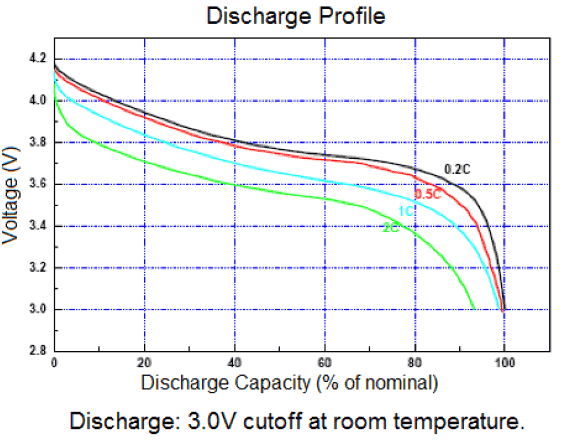
\includegraphics[width=11cm]{billeder/discharge_curve.png}
\caption{Genereliseret afladningskurve for en lithium-ion celle}
\label{fig:discharge_curve}
\end{figure}

Her kan det ses at spændingen på batterierne falder i takt med at de aflades. Denne kurve er dog ikke lineær og varierer fra celle til celle, og specielt mellem forskellige kemier. Der ses også at jo hårdere der afladers, jo mindre kapacitet kan der udvindes. På denne specifikke graf fås et optimalt udbytte af cellen hvis der aflades med 1C, uden at gå på kompromis med hverken afladekapacitet eller samlet energiudbytte. \\

"Sikkerhedszonen" \space er også i spil her. Hvis der aflades med for eksempel $0.2C$, og afladningen stoppes ved omkring de $3.2\volt$, udvindes det meste af cellens kapacitet, mens der sørges for at cellen har så lang en levetid som muligt. Her er det dog nødvendigt at gå lidt på kompromis med afladekapaciteten, for hvis der aflades med f.eks. $2C$, er der teoretisk set stadig omkring $88-90\percent$ kapacitet tilbage som der ikke kan blive brugt uden at cellen tager skade i det lange forløb. \\

Skal cellerne opbevares i længere tid, er det en god idé at opbevare dem i den såkaldte "storage mode". Her lades/aflades cellerne til $30-40\percent$ af deres fulde kapacitet, da der her er mindst slid, og man derfor opnår en længere levetid. 

\section{Sikkerhed}
Da lithium batterier kan være farlige, er det nødvendigt til at foretage de nødvendige sikkerhedsforanstaltninger. Derfor er der en del "regler":

\begin{itemize}[noitemsep]
\item Oplad ikke på batteriet når omgivelsestemperaturen er under $0\degreeCelsius$ eller over $45\degreeCelsius$. 
\item Aflad ikke batteriet når omgivelsestemperaturen er under $-20\degreeCelsius$ eller over $60\degreeCelsius$.
\item Batteriet må ikke oplades til mere end $4.2\volt$ ($3.65\volt$ når det er $LiFePO_4$).
\item Brug helst en balance oplader eller et batteristyresystem, hvis der er flere celler i serie.
\end{itemize}

Når der udvilkles systemer med lithium-ion batterier er det en god ide at batteristyresystemet indeholder kortslutningsbeskyttelse og op- og afladningskontrol. Med dette kan der undgås at aflade cellerne for hårdt og/eller en direkte kortslutning af cellerne. Det er også en god idé at have temperatursensorer i systemet for at overvåge cellernes temperatur samt omgivelsestemperaturerne (se ovenstående punkter). Dette er med til at forøge cellernes levetid. 

%\section{Ækvivalent kredsløbs model af en celle (ECM)}
%For at kunne udvikle et batteristyresystem er det nødvendigt, at have en model for en celle i form at et elektrisk ækvivalensdiagram. Alt afhængig af modellens kompleksitet vil databehandling af State of Charge og State of Health blive mere præcis. \\
%
%Den mest simple model kan tilnærme sig op- og afladningskarakteristikken for en superkondensator, hvor kurven er lineær gennem hele arbejdsområdet. \\
%
%\begin{figure}[h]
%	\centering
%	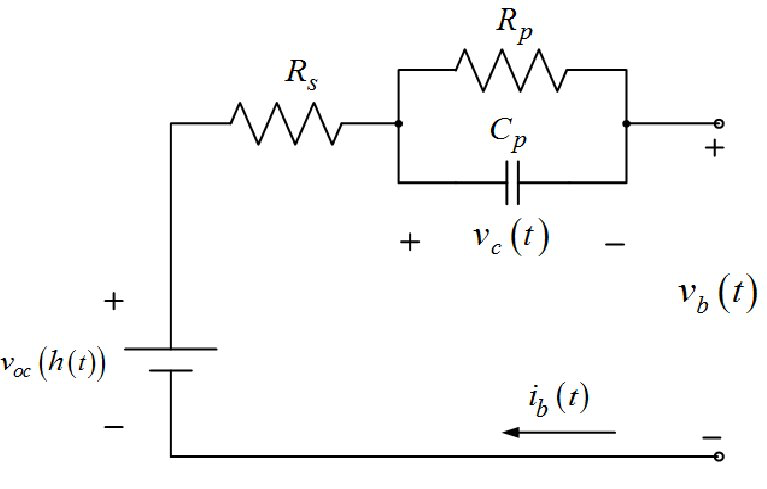
\includegraphics[width=9cm]{billeder/ecm.png}
%	\caption{Elektrisk ækvivalensdiagram for en lithium-ion celle}
%	\label{fig:ecm}
%\end{figure}




